\documentclass[11pt,aspectratio=169]{beamer}
\usetheme{metropolis}
\usepackage[T1]{fontenc} 
\usepackage{dirtytalk}
\usepackage{tabularx}
\usepackage[superscript,biblabel]{cite}
\usecolortheme[snowy]{owl}
% \setsansfont{JetBrains Mono}
%\setbeamertemplate{navigation symbols}{}
% \setbeamercovered{transparent}
\title {Linux Foundation}
\author{Stefan Fürst}
\institute{Htl Donaustadt}
% \logo{
\includegraphics[width=.1\textwidth]{logo.png}}
\begin{document}

\begin{frame}
	\maketitle
\end{frame}

\begin{frame}{Inhaltsverzeichnis}
	\tableofcontents
\end{frame}
\section{Was ist die Linux Foundation?}
\begin{frame}{Was ist die Linux Foundation?}
	\begin{itemize}
		\item Gemeinnütziges Konsortium \cite{NPO}
		\item Zusammenschluss aus der Free Standards Group und Open Souce Development Labs\cite{Zusamenschluss}
	\end{itemize}
\end{frame}
\section{Was macht die Linux Foundation?}

\begin{frame}{Was macht die Linux Foundation?}
	\begin{itemize}
		\item<1-> Mit eigenen Worten:\say{Empowering generations of open source innovators.}\cite{About}
		\item<2-> Open Source Projekte Untersützen
		\item<3-> für offene Standarts Einsetzen
		\item <4->entwicklung von Linux untersützen
		\item<5-> Events Organisieren\cite{Events}
		\item<6-> Entwickler ausbilden\cite{Training}
	\end{itemize}

\end{frame}

\begin{frame}{Wie macht sie das?}
	\begin{itemize}
		\item <1->\say{Foundation as a Service}
		\item <2->Finanzielle Untertützung
		\item <3->Rechtlicher Schutz
		\item <4->Lernmaterialien und Zertifizirungen anbieten\cite{Training}
	\end{itemize}
\end{frame}
\begin{frame}{Wieso ist das wichtig?}
	\begin{itemize}	
		\item Offene Standarts
	\end{itemize}
	\begin{itemize}	
		\item Offene Software
	\end{itemize}
\end{frame}
\begin{frame}{HDMI Situation}
	\begin{itemize}	
		\item HDMI ist ein kein offender Standard
		\begin{itemize}	
			\item Nur "HDMI Adopters" haben zugriff
		\end{itemize}
		\item 
	\end{itemize}
\end{frame}
\begin{frame}{Open Source}
	\begin{itemize}
		\item \say{Die Welt braucht nicht mehr Windowse}
	\end{itemize}
\end{frame}
\begin{frame}{Wo macht sie das?}
	\begin{itemize}
		\item Weltweit mit Sitzen in:
		      \begin{itemize}
			      \item Hauptsitz in San Francisco \cite{Locations}
			      \item Sitz in Japan\cite{Locations}
			      \item Sitz in Belgien\cite{Locations}
		      \end{itemize}
	\end{itemize}
\end{frame}
\begin{frame}{Gesuchte Stellen}
	\begin{itemize}

		\item	Hauptsächlich Managment Positionen
	\end{itemize}
	\begin{figure}
		\centering
		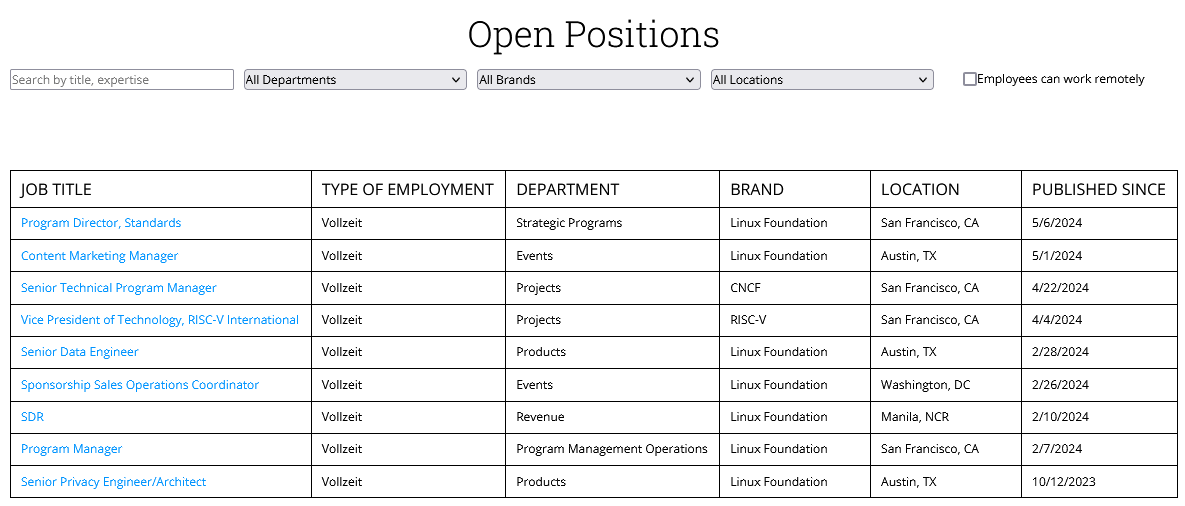
\includegraphics[scale=0.4]{images/jobs.png}\cite{Positionen}
		\caption{Offene Stellen}
	\end{figure}

\end{frame}
\section {Ziele der Firma}
\begin{frame}{Hauptziele}
	\begin{itemize}
		\item <1-> Hauptziele
		      \begin{itemize}

			      \item<2->Grundprinzipien folgen\cite{Grundprinziepe}
			            \begin{itemize}
				            \item<3-> Organisatorische Neutralität
				            \item<4-> Klare Trennung von Finanzierung und Beteiligung
				            \item<5-> Open Governance
				            \item<6-> Klarheit des geistigen Eigentums
				            \item<7-> Kommerzielles Support-Ökosystem
				            \item<8-> Alle Finanzen stammen aus Spenden und Sponsoring
			            \end{itemize}
		      \end{itemize}
	\end{itemize}
\end{frame}
\begin{frame}{Nebenziele}
	\begin{itemize}
		\item Nebenziele
		      \begin{itemize}
			      \item Sponsorings von Firmen eintreiben
			      \item Sämtliche andere Monitäre Ziele
		      \end{itemize}
	\end{itemize}
\end{frame}
\subsection {Monetäre und nicht monetäre Ziele}
\begin{frame}{Monetäre und nicht monetäre Ziele}
	\begin{itemize}
		\item Monetär
		      \begin{itemize}
			      \item Sponsoren finden
			      \item Kurse und Zertifikate Verkaufen\cite{Training}
		      \end{itemize}
		      \begin{itemize}
			      \item nicht monetär
			            \begin{itemize}
				            \item Grundprenzipien und Mission folgen\cite{Grundprinziepe}
			            \end{itemize}
		      \end{itemize}
	\end{itemize}
\end{frame}

\subsection {komplementäre und konkurierende Ziele}
\begin{frame}{komplementäre und konkurierende Ziele}
	\begin{itemize}
		\item komplementär
		      \begin{itemize}
			      \item Open Source Community Untersützen und Events Hosten
		      \end{itemize}
	\end{itemize}
	\begin{itemize}
		\item konkurierend
		      \begin{itemize}
			      \item Durch Einhaltung der Grundprinzipien weniger möglichkeiten an Kapital zu kommen
		      \end{itemize}
	\end{itemize}
\end{frame}

\subsection {Haupt und Nebenziele}

\section{Quellen}
\begin{frame}[shrink=30]{Quellen}
	\bibliographystyle{plain}
	\bibliography{./quellen.bib}
\end{frame}
\begin{frame}{ende oida}
	\LaTeX{} > Powerpoint microsoft bad
\end{frame}

\end{document}
